%!TEX root = ../../main.tex

% Processo de aprendizado OK
% Tarefa de classificação binária
% Divisão dos Dados
% Explicação do método holdout
% Parâmetros e hiperparâmetros
% Métricas Utilizadas - cenários balanceados e desbalanceados


Com o intuito de checar a autenticidade de assinaturas utilizando CNNs, concebeu-se uma tarefa de classificação binária para alcançar este objetivo. Nela, uma imagem de $256 \times 256$ \emph{pixels} composta por duas assinaturas manuscritas, na qual a primeira delas representa uma assinatura de referência genuína e a segunda compreende uma assinatura a ser verificada. A partir desta entrada, deseja-se obter como a saída de uma CNN para esta tarefa, a predição da autenticidade da segunda assinatura que, por ser uma tarefa de classificação binária, poderá assumir somente duas classificações: \emph{autêntica} ou \emph{forjada}. Os passos compreendidos nesta tarefa podem ser visualizados na Figura \ref{fig:esquema-solucao}.

\begin{figure}[h!]
  \centering
  \caption{Uma visão geral da tarefa de aprendizado considerada.}
  \label{fig:esquema-solucao}
  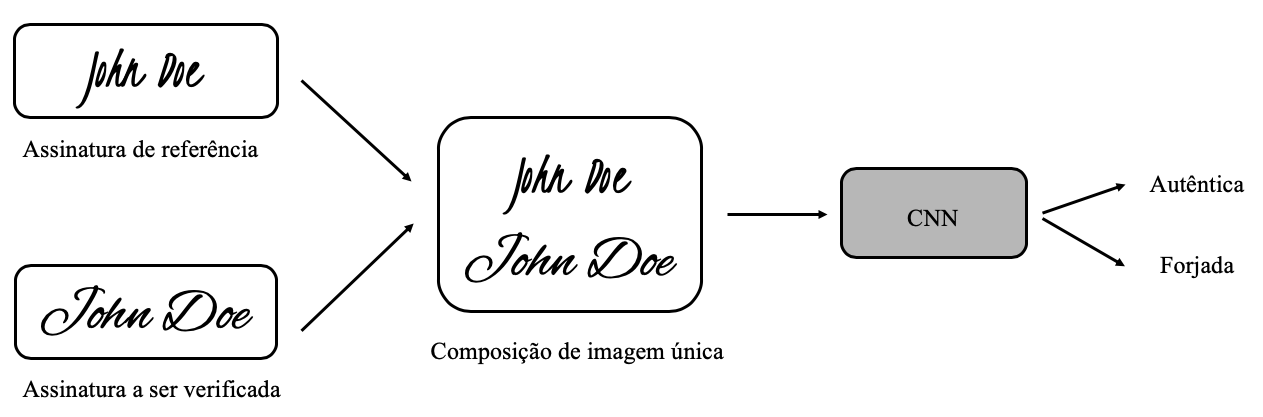
\includegraphics[width=\textwidth]{imgs/esquema-solucao}
\end{figure}

Para esta tarefa, diferentes CNNs serão consideradas. O treinamento e teste destes modelos serão feitos com o método \emph{holdout} de validação cruzada, em que $70\%$ dos dados serão utilizados no treino e ajuste de parâmetros, enquanto $20\%$ dos dados serão aproveitados para o processo de teste das redes, com vista a capturar o poder de generalização dos modelos considerados. Os $10\%$ de dados remanescentes, serão utilizados para a validação dos modelos durante o processo de treinamento \cite{brink}.

Os modelos propostos serão avaliados perante as métricas de desempenho de \emph{Acurácia} e \emph{F-score}. A acurácia indica a proporção de predições corretas inferidas pelos modelos. O \emph{F-score}, por sua vez, será calculado pela média harmônica da precisão e da revocação considerando uma tarefa de classificação binária \cite{marsland}, da seguinte forma:

\begin{equation*}
\textrm{Precisão} = \frac{TP}{TP + FP}, \hspace{2cm} \textrm{Revocação} = \frac{TP}{TP + FN},
\end{equation*}


\begin{eqnarray*}
\textrm{F-Score} &=&  2\cdot \frac{\textrm{Precisão} \times \textrm{Revocação}}{\textrm{Precisão} + \textrm{Revocação}},
\end{eqnarray*} em que $TP$ indica o número de verdadeiros positivos, $FP$ indica o número de falsos positivos e $FN$ indica o quantitativo de falsos negativos nas previsões obtidas.
